\documentclass[aspectratio=169]{beamer}
\usetheme{SimplePlus}

\usepackage{tikz}
\usepackage{pgfplots}
\pgfplotsset{compat=1.17}
\usepackage{mathtools}
\usepackage{isomath}
\usepackage{centernot}
\usepackage{amsmath, amssymb, amsthm, bm}
\DeclareMathOperator{\grad}{\nabla}
\renewcommand{\P}{\mathbb{P}}
\newcommand{\R}{\mathbb{R}}
\newcommand{\ttag}[1]{(#1)}

\newcommand{\ten}{\tensorsym}
\renewcommand{\vec}{\vectorsym}

\title[Continuum Mechanics]{Kinematics of Continuum Mechanics}
\author{Nicol\'as A. Barnafi}
\date{\today}

\begin{document}

\begin{frame}
    \titlepage
\end{frame}

\section{Kinematics and Configurations}

\begin{frame}{Continuum mechanics}
    Tracking \textbf{reference configuration} $\Omega_0$ to its \textbf{current configuration} $\Omega_t$ at time $t$.

    \begin{center}
    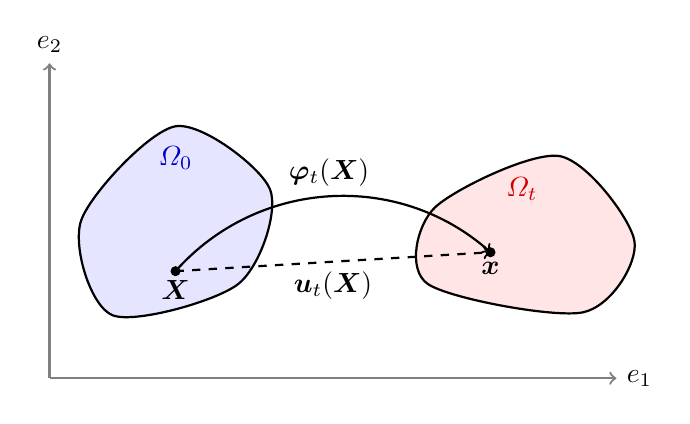
\begin{tikzpicture}[scale=0.8]
        % Axes
        \draw[->, thick, gray] (-1,-1) -- (8,-1) node[right, black] {$e_1$};
        \draw[->, thick, gray] (-1,-1) -- (-1,4) node[above, black] {$e_2$};

        % Reference configuration (Potato 1)
        \draw[thick, fill=blue!10, smooth cycle] plot coordinates {(0,0) (2,0.5) (2.5,2) (1,3) (-0.5,1.5)};
        \node[blue!80!black] at (1,2.5) {$\Omega_0$};

        % Current configuration (Potato 2)
        \draw[thick, fill=red!10, smooth cycle, xshift=5cm, yshift=0.5cm, rotate=-15] plot coordinates {(0,0) (2.5,0.2) (3,1.5) (1.5,2.5) (-0.2,1.2)};
        \node[red!80!black] at (6.5,2.0) {$\Omega_t$};

        % Points
        \filldraw (1, 0.7) circle (2pt) node[below] {$\bm{X}$};
        \filldraw (6, 1) circle (2pt) node[below] {$\bm{x}$};

        % Vectors
        %\draw[->, thick] (-1,-1) -- (1,0.5) node[midway, above left] {$\bm{X}$};
        %\draw[->, thick] (-1,-1) -- (6,1) node[midway, below right] {$\bm{x}$};

        % Mapping
        \draw[->, thick, bend left=45] (1,0.7) to node[above] {$\bm{\varphi}_t(\bm{X})$} (6,1);
        \draw[->, thick, dashed] (1,0.7) -- (6,1) node[midway, below] {$\bm{u}_t(\bm{X})$};
    \end{tikzpicture}
    \end{center}

    The \textbf{deformation map} $\bm{\varphi}$ is injective, orientation-preserving ($\det \nabla_{\bm{X}} \bm{\varphi} > 0$) mapping \emph{reference/material} coordinates $\bm{X}$ to \emph{spatial/deformed} coordinates $\bm{x} = \bm{\varphi}_t(\bm{X})$. 

    The \textbf{displacement} is $\bm{u}_t(\bm{X}) = \bm{x} - \bm{X}$.
\end{frame}

\section{Deformation Metrics}

\begin{frame}{Deformation Metrics: Measuring Stretch and Strain}
    How do infinitesimal elements deform? $d\bm{x} = \bm{\varphi}_t(\bm{X} + d\bm{X}) - \bm{\varphi}_t(\bm{X}) \approx \nabla_{\bm{X}}\bm{\varphi}_t(\bm{X}) d\bm{X}$.

    \begin{itemize}[<+->]
        \item \textbf{Deformation Gradient Tensor ($\ten F$):} Maps material line elements to spatial ones.
        $$ \ten F = \nabla_{\bm{X}} \bm{\varphi}_t = I + \nabla_{\bm{X}} \bm{u}_t \quad \implies \quad d\bm{x} = \ten F d\bm{X} $$

        \item \textbf{Right Cauchy-Green Tensor ($\ten C$):} Measures changes in squared lengths.
        $$ \|d\bm{x}\|^2 = d\bm{x}^T d\bm{x} = (\ten F d\bm{X})^T (\ten F d\bm{X}) = d\bm{X}^T (\ten F^T \ten F) d\bm{X} \quad \implies \quad \ten C = \ten F^T \ten F $$

        \item \textbf{Euler-Lagrange Strain Tensor ($\ten E$):} Measures exact strain.
        $$ \|d\bm{x}\|^2 - \|d\bm{X}\|^2 = d\bm{X}^T (\ten C - \ten I) d\bm{X} = 2 d\bm{X}^T \ten E d\bm{X} \quad \implies \quad \ten E = \frac{1}{2}(\ten C - \ten I) $$

        \item \textbf{Infinitesimal Strain Tensor ($\bm{\varepsilon}$):} The linearization of $\ten E$ for small displacements.
        $$ \ten E = \frac{1}{2}(\nabla_{\bm{X}} \bm{u} + (\nabla_{\bm{X}} \bm{u})^T + (\nabla_{\bm{X}} \bm{u})^T \nabla_{\bm{X}} \bm{u}) \quad \xrightarrow{\text{small } \nabla \bm{u}} \quad \bm{\varepsilon} = \frac{1}{2}(\nabla_{\bm{X}} \bm{u} + (\nabla_{\bm{X}} \bm{u})^T) $$
    \end{itemize}
\end{frame}

\section{Explicit Example}

\begin{frame}{An Explicit Example: Simple Shear}
    Consider a simple shear deformation given by $\bm{x} = \bm{X} + \gamma X_2 \bm{e}_1$, then $\bm{u} = \gamma X_2 \bm{e}_1$.

    \begin{columns}
        \begin{column}{0.4\textwidth}
            \begin{center}
            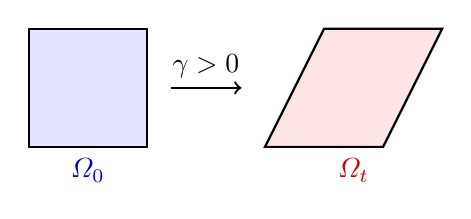
\begin{tikzpicture}[scale=1.5]
                \draw[thick, fill=blue!10] (0,0) rectangle (1,1);
                \node[blue!80!black] at (0.5,-0.2) {$\Omega_0$};

                \draw[->, thick] (1.2, 0.5) -- (1.8, 0.5) node[midway, above] {$\gamma > 0$};

                \draw[thick, fill=red!10] (2,0) -- (3,0) -- (3.5,1) -- (2.5,1) -- cycle;
                \node[red!80!black] at (2.75,-0.2) {$\Omega_t$};
            \end{tikzpicture}
            \end{center}
            The gradient of the displacement is:
            $$ \nabla_{\bm{X}} \bm{u} = \begin{pmatrix} 0 & \gamma & 0 \\ 0 & 0 & 0 \\ 0 & 0 & 0 \end{pmatrix} $$
        \end{column}
        \begin{column}{0.6\textwidth}
            \begin{align*}
                \ten F &= I + \nabla_{\bm{X}} \bm{u} &=& \begin{pmatrix} 1 & \gamma & 0 \\ 0 & 1 & 0 \\ 0 & 0 & 1 \end{pmatrix} \\
                \ten C &= F^T F &=& \begin{pmatrix} 1 & \gamma & 0 \\ \gamma & 1+\gamma^2 & 0 \\ 0 & 0 & 1 \end{pmatrix} \\
                \ten E &= \frac{1}{2}(C - I) &=& \begin{pmatrix} 0 & \gamma/2 & 0 \\ \gamma/2 & \alert{\gamma^2/2} & 0 \\ 0 & 0 & 0 \end{pmatrix} \\
                \bm{\varepsilon} &= \frac{1}{2}(\nabla_{\bm{X}} \bm{u} + \nabla_{\bm{X}} \bm{u}^T) &=& \begin{pmatrix} 0 & \gamma/2 & 0 \\ \gamma/2 & \alert{0} & 0 \\ 0 & 0 & 0 \end{pmatrix}
            \end{align*}
        \end{column}
    \end{columns}
\end{frame}

\section{Principal Directions and Differentials}

\begin{frame}{Principal Directions and Invariants}
    \textbf{Principal Stretches:} Given a material direction $\bm{m}$, consider $d\vec X = \| d\vec X\| \vec m$, define the stretch ration
    $$ \Delta(\bm{m}) := \frac{\|d\bm{x}\|^2}{\|d\bm{X}\|^2} = \bm{m}^T C \bm{m} $$
    Maximum stretch $\max_{\vec m}\Delta(\bm{m})$ leads to the eigenvalue problem $\ten C\bm{m} = \lambda \bm{m}$. \emph{Principal stretches} $\lambda_i > 0$ and \emph{principal directions} $\bm{m}_i$.

    \vspace{0.3cm}
    \textbf{Tensor Invariants:} Quantities independent of the coordinate system (i.e., $I(QAQ^T) = I(A)$). For $C$, these are:
    \begin{align*}
        I_1(C) &= \text{tr}(C) = \lambda_1 + \lambda_2 + \lambda_3 \\
        I_2(C) &= \text{tr}(\text{Cof}(C)) = \lambda_1\lambda_2 + \lambda_1\lambda_3 + \lambda_2\lambda_3 \\
        I_3(C) &= \det(C) = \lambda_1\lambda_2\lambda_3 = J^2 \quad (\text{where } J = \det F)
    \end{align*}
\end{frame}

\begin{frame}{Algebra of Differentials: Nanson's Formula}
    \begin{itemize}
        \item Before we saw mapping of linear elements $d\vec x= \ten F d\vec X$. 
        \item Jacobian $J = \det F$ dictates the transformation of volume elements: $dv = J dV$.
        \item Area $d\vec a$ from $d\vec A$...? \textbf{Nanson's Formula}.
    \end{itemize}

    \vspace{0.2cm}
    $$ d\vec a = \bm{n} da = J \ten F^{-T} \bm{N} dA = d\vec A $$

    In particular,

    $$ \vec n = \frac{J \ten F^{-T}\vec N}{\|J \ten F^{-T} \vec N\|}$$

\end{frame}

\section{Velocities and Derivatives}

\begin{frame}{Velocities and the Material Derivative}
    \begin{itemize}
        \item \textbf{Material quantities}: $\eta(\vec X, t)$
        \item \textbf{Spatial quantities}: $\eta(\vec x, t)$
    \end{itemize}

    \pause Velocities:
    \begin{itemize}
        \item \textbf{Material Velocity:} $\bm{V}(\bm{X}, t) = \frac{\partial \bm{\varphi}(\bm{X}, t)}{\partial t}$.
        \item \textbf{Spatial Velocity:} $\bm{v}(\bm{x}, t) = \bm{V}(\bm{\varphi}_t^{-1}(\bm{x}))$.
    \end{itemize}

    For a spatial scalar field $\psi(\bm{x}, t)$, the total time derivative experienced by a moving particle is given by the \textbf{Material Derivative}:

    $$ \frac{D\psi}{Dt} = \frac{\partial \psi}{\partial t} + \nabla_{\bm{x}} \psi \cdot \frac{\partial \bm{x}}{\partial t} \quad \implies \quad \frac{D\psi}{Dt} = \frac{\partial \psi}{\partial t} + \bm{v} \cdot \nabla_{\bm{x}} \psi $$

\end{frame}

\begin{frame}{Tensor Derivative Identities}
    To perform rigorous analysis and derive conservation laws, several core identities regarding the tensor calculus of kinematics are required. Let $L = \nabla_{\bm{x}} \bm{v}$ be the spatial velocity gradient.

    \vspace{0.3cm}
    \textbf{1. Time derivative of the deformation gradient:}
    $$ \dot{F} = L_m F \quad (\text{where } L_m(\bm{X},t) = L(\bm{\varphi}(\bm{X},t), t)) $$

    \textbf{2. Derivative of a determinant:}
    $$ \frac{\partial(\det A)}{\partial A} = \text{Cof}(A) = (\det A) A^{-T} $$

    \textbf{3. Euler's Expansion Formula (Time derivative of the Jacobian):}
    $$ \dot{J} = \text{Cof}(F) : \dot{F} = J (F^{-T} : L_m F) = J \, \text{tr}(L_m) = J \text{div}_{\bm{x}} \bm{v} $$
\end{frame}

\section{The Piola Identity}

\begin{frame}{Concluding Proof: The Piola Identity}
    \begin{block}{Piola Identity}
        $$ \text{Div}_{\bm{X}} (\text{Cof}(\ten F)) = 0 \quad \text{or equivalently} \quad \text{Div}_{\bm{X}} (J \ten F^{-T}) = 0 $$
    \end{block}

    \pause
    \textbf{Proof:} \\
    By localization, consider an arbitrary $\omega_0 \subset \Omega_0$ mapped to $\omega_t \subset \Omega_t$. Integrating:
    \begin{align*}
        \int_{\omega_0} \text{Div}_{\bm{X}} (J F^{-T}) dV &= \int_{\partial \omega_0} (J F^{-T}) \bm{N} dA \tag{Divergence Theorem on $\omega_0$} \\
        &= \int_{\partial \omega_t} \bm{n} da \tag{Nanson's Formula} \\
        &= \int_{\omega_t} \text{div}_{\bm{x}} (1) dv \tag{Divergence Theorem on $\omega_t$} \\
        &= \int_{\omega_t} 0 \, dv = 0
    \end{align*}
    Since the integral is zero for any arbitrary arbitrary subdomain $\omega_0$, we conclude. \qed
\end{frame}

\end{document}
